\documentclass{beamer}
\usepackage[utf8]{inputenc}

\usetheme{Madrid}
\usecolortheme{default}
\usepackage{amsmath,amssymb,amsfonts,amsthm}
\usepackage{txfonts}
\usepackage{tkz-euclide}
\usepackage{listings}
\usepackage{adjustbox}
\usepackage{array}
\usepackage{tabularx}
\usepackage{gvv}
\usepackage{lmodern}
\usepackage{circuitikz}
\usepackage{tikz}
\usepackage{graphicx}

\setbeamertemplate{page number in head/foot}[totalframenumber]

\usepackage{tcolorbox}
\tcbuselibrary{minted,breakable,xparse,skins}



\definecolor{bg}{gray}{0.95}
\DeclareTCBListing{mintedbox}{O{}m!O{}}{%
  breakable=true,
  listing engine=minted,
  listing only,
  minted language=#2,
  minted style=default,
  minted options={%
    linenos,
    gobble=0,
    breaklines=true,
    breakafter=,,
    fontsize=\small,
    numbersep=8pt,
    #1},
  boxsep=0pt,
  left skip=0pt,
  right skip=0pt,
  left=25pt,
  right=0pt,
  top=3pt,
  bottom=3pt,
  arc=5pt,
  leftrule=0pt,
  rightrule=0pt,
  bottomrule=2pt,
  toprule=2pt,
  colback=bg,
  colframe=orange!70,
  enhanced,
  overlay={%
    \begin{tcbclipinterior}
    \fill[orange!20!white] (frame.south west) rectangle ([xshift=20pt]frame.north west);
    \end{tcbclipinterior}},
  #3,
}
\lstset{
    language=C,
    basicstyle=\ttfamily\small,
    keywordstyle=\color{blue},
    stringstyle=\color{orange},
    commentstyle=\color{green!60!black},
    numbers=left,
    numberstyle=\tiny\color{gray},
    breaklines=true,
    showstringspaces=false,
}
%------------------------------------------------------------
%This block of code defines the information to appear in the
%Title page
\title %optional
{2.2.24}
\date{August 31,2025}


\author 
{Jnanesh Sathisha karmar - EE25BTECH11029}



\begin{document}



\frame{\titlepage}
\begin{frame}{Question}
Show that the points $\brak{1, 7}$, $\brak{4, 2}$, $\brak{-1, -1}$ and $\brak{-4, 4}$ are the vertices of a square.
\end{frame}



\begin{frame}{Equation}
For the points $\vec{ABCD}$ to represent a square:
\begin{align}
    \norm{AB}=\norm{BC}=\norm{CD}=\norm{DA}\\
    \angle{BAD}=\angle{ABC}=\angle{DCA}=\angle{ADC}=90
\end{align}
\end{frame}
\begin{frame}{Theoretical Solution}

Given details:
\begin{align}
    \vec{A}=\myvec{1\\7}  \vec{B}=\myvec{4\\2} \vec{C}=\myvec{-1\\-1} \vec{D}=\myvec{-4\\4}
\end{align}
\end{frame}

\begin{frame}{Theoretical Solution}

Find the sides
\begin{align}
\vec{AB}=\vec{B}-\vec{A}=\myvec{3\\-5} \  \vec{BC}=\vec{C}-\vec{B}=\myvec{-5\\-3} \\
\vec{CD}=\vec{D}-\vec{C}=\myvec{-3\\5} \ 
\vec{DA}=\vec{A}-\vec{D}=\myvec{5\\3}
\end{align}

\end{frame}


\begin{frame}{Theoretical Solution}
Check side lengths
\begin{align}
    \norm{AB}=\sqrt{\vec{AB}^T\vec{AB}}=\sqrt{3^2+\brak{-5}^2}=\sqrt{34}\\
    \norm{BC}=\sqrt{\vec{BC}^T\vec{BC}}=\sqrt{\brak{-5}^2+\brak{-3}^2}=\sqrt{34}\\
    \norm{CD}=\sqrt{\vec{CD}^T\vec{CD}}=\sqrt{\brak{-3}^2+5^2}=\sqrt{34}\\
    \norm{DA}=\sqrt{\vec{DA}^T\vec{DA}}=\sqrt{5^2+3^2}=\sqrt{34}
\end{align}
\end{frame}
\begin{frame}{Theoretical Solution}
Therefore all the sides are of equal length
\begin{align}
    \norm{AB}=\norm{BC}=\norm{CD}=\norm{DA}
\end{align}
\end{frame}
\begin{frame}{Theoretical Solution}
Condition for right angle:
For two sides to be angled at 90 the Dot product between the 2 side vectors should be 0
\begin{align}
    =\vec{AB^TBC}=\brak{3}\brak{5}+\brak{-5}\brak{-3}=-15+15=0
\end{align}
Therefore the sides are perpendicular to each other\\
Since all the sides are equal and one of the angles is 90 , all the points represent a square.
\end{frame}

\begin{frame}[fragile]
    \frametitle{C Code (1) - Function to store the points }

    \begin{lstlisting}

#include <stdio.h>

// Fill the array with square vertices: A(1,7), B(4,2), C(-1,-1), D(-4,4)
void get_square_points(double *points) {
    double coords[8] = {1,7,  4,2,  -1,-1,  -4,4};

    for (int i = 0; i < 8; i++) {
        points[i] = coords[i];
    }
}

    \end{lstlisting}
\end{frame}


\begin{frame}[fragile]
    \frametitle{Python Code - Using Shared Object}
    \begin{lstlisting}

import ctypes
import numpy as np
import matplotlib.pyplot as plt

# Load the shared object
square_lib = ctypes.CDLL("./square.so")

# Define function return type
square_lib.get_square_points.argtypes = [np.ctypeslib.ndpointer(dtype=np.double, ndim=1, flags="C")]


\end{lstlisting}
\end{frame}

\begin{frame}[fragile]
    \frametitle{Python Code - Using Shared Object}
    \begin{lstlisting}
# Create numpy array to hold 8 values (x,y for 4 points)
points = np.zeros(8, dtype=np.double)

# Call C function to fill points
square_lib.get_square_points(points)

# Reshape into (4,2)
points = points.reshape((4,2))

# Close the square (repeat first point)
points = np.vstack([points, points[0]])

\end{lstlisting}
\end{frame}
\begin{frame}[fragile]
    \frametitle{Python Code - Using Shared Object}
    \begin{lstlisting}
# Plot square
plt.plot(points[:,0], points[:,1], "bo-")
plt.title("Square from C library")
plt.xlabel("X")
plt.ylabel("Y")
plt.gca().set_aspect("equal")
plt.grid(True)
plt.savefig('figs/square.png')
subprocess.run(shlex.split("termux-open figs/sqaure.png")






\end{lstlisting}
\end{frame}



\begin{frame}{Plot-Using Both C and Python}
    \centering
    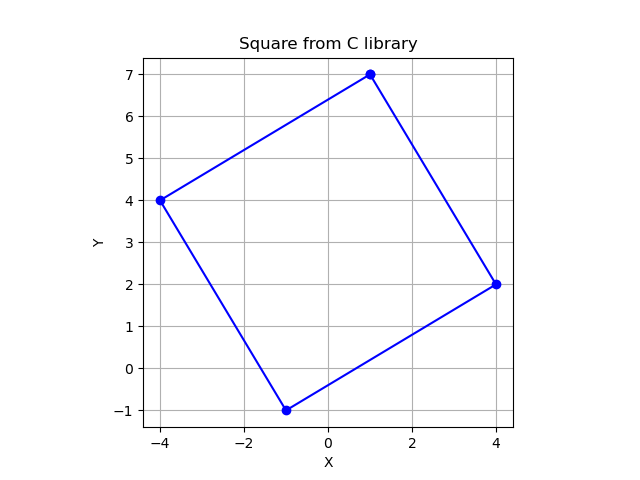
\includegraphics[width=\columnwidth, height=0.8\textheight, keepaspectratio]{figs/square.png}     
\end{frame}

\begin{frame}[fragile]
    \frametitle{Python Code}
    \begin{lstlisting}
import numpy as np
import matplotlib.pyplot as plt

# Define the square vertices
points = np.array([
    [1, 7],   # A
    [4, 2],   # B
    [-1, -1], # C
    [-4, 4]   # D
])




\end{lstlisting}
\end{frame}

\begin{frame}[fragile]
    \frametitle{Python Code }
    \begin{lstlisting}
# Close the square (repeat first point)
points = np.vstack([points, points[0]])

# Plot
plt.plot(points[:,0], points[:,1], "bo-", linewidth=2)
plt.title("Square of 4 Points")
plt.xlabel("X-axis")
plt.ylabel("Y-axis")
plt.gca().set_aspect("equal")
plt.grid(True)
plt.savefig('figs/square2.png')
subprocess.run(shlex.split("termux-open figs/distance.png")



\end{lstlisting}
\end{frame}





\begin{frame}{Plot-Using only Python}
    \centering
    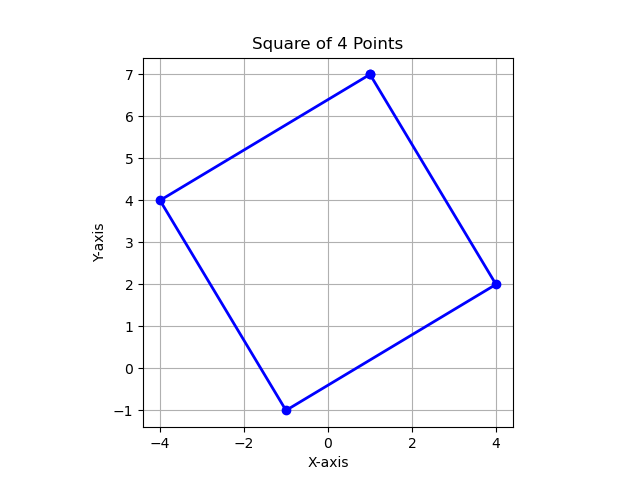
\includegraphics[width=\columnwidth, height=0.8\textheight, keepaspectratio]{figs/square2.png}     
\end{frame}


\end{document}